\PassOptionsToPackage{unicode}{hyperref}
\PassOptionsToPackage{naturalnames}{hyperref}
\documentclass[12pt, xetex, xcolor=pdftex, dvipsnames]{beamer}
\usetheme{metropolismyfont}
\usepackage{dcolumn} % for apsrtable outputs
\usepackage{xunicode} % extra support for unicode
\usepackage{xltxtra} % implements some odds-and-ends features
\usepackage{verbatim} % for multiple-line comments
% to fix a problem in line-breaks
% see "http://zrbabbler.hp.infoseek.co.jp/xelatex.html"
\XeTeXlinebreaklocale "ja"
\XeTeXlinebreakskip=0pt plus 1pt
\XeTeXlinebreakpenalty=0
\def\<{\@ifstar{\zx@hwback\nobreak}{\zx@hwback\relax}}
\def\zx@hwback#1{\leavevmode#1\hskip-.5em\relax}

\renewcommand{\vec}{\textbf} %\vecを矢印からボールドに
\usepackage{color}
\usepackage{listings}
\lstset{%
    language={Python},%
    basicstyle={\footnotesize},%
    identifierstyle={\footnotesize},%
    commentstyle={\footnotesize\color{mLightGreen}},%
    keywordstyle={\footnotesize\color{mLightBrown}},%
    stringstyle={\footnotesize\color{mDarkBrown}},%
    frame={tblr}%
}

\usepackage{graphicx}

\AtBeginSection[]{
    \begin{frame}{目次}
        \setbeamertemplate{section in toc}[sections numbered]
        \tableofcontents[currentsection, hideallsubsections]
    \end{frame}
}

\title{引き継ぎ資料 Vol.6}
\subtitle{全曲率の話}
\date{2016/09/??}
\author{}
\institute{}
\begin{document}
\maketitle
\begin{frame}{コンセプト}
    \alert{\textbf{ソースとテクニックを同時に話そう}}
\end{frame}

\begin{frame}{目次}
  \setbeamertemplate{section in toc}[sections numbered]
  \tableofcontents[hideallsubsections]
\end{frame}

\section{概要}
\begin{frame}{やりたいこと}
\textbf{{\large 3次元軌道からS字を抽出}}
\end{frame}
\begin{frame}{やりかた}
    \begin{itemize}
        \item \only<1,3>{モーキャプデータをB-splineとして近似}\only<2>{({\small モーキャプデータをB-splineとして近似})}
        \item 軌道を投影し2次元化
        \item S字の抽出\only<3>{
            \begin{itemize}
                \item 変曲点の計算
                \item 全曲率が一定となるように取り出し
            \end{itemize}
        }
    \end{itemize}
\end{frame}

\section{軌道の3次元関数}
\begin{frame}{B-spline曲線}
    B-spline曲線の詳細は省略
    \begin{align}
        \vec{B}(t) (0\leq t \leq 1)
    \end{align}
    $\vec{B}(t)$はtを媒介変数とする3次元曲線
\end{frame}
\begin{frame}[fragile]{実装的な話}
\begin{itemize}
\item Bは関数名
\item 3次元の座標を返す
\end{itemize}
\begin{lstlisting}
>>> B(0.)
array([0., 0., 0.])
\end{lstlisting}
\end{frame}

\section{2次元化}
\begin{frame}{理論}
    \begin{align}
        \vec{P}(t) = M \cdot \vec{B}(t)
    \end{align}

    $M$が$2 \times 3$の行列なら$\vec{P}(t)$は2次元軌道
\end{frame}
\begin{frame}[fragile]{実装}
クラスを一つ作成
\begin{lstlisting}
class SecondDimensionalize:
    def __init__(self, func):
        self.mat = np.array(
            [[1.0, 0.0, 0.0],
             [0.0, 1.0, 0.0]]
        )
        self.func = func

    def __call__(self, t):
        return np.dot(self.mat, self.func(t))
\end{lstlisting}
\end{frame}
\begin{frame}[fragile]{実装}
見かけ上関数に見えるオブジェクト

\begin{lstlisting}
>>> p = SecondDimensionalize(B)
>>> p(0.)
array([0., 0.])
\end{lstlisting}
\end{frame}
\begin{frame}
    なぜ見かけ上関数に見えるオブジェクトが必要?

    \pause

    \alert{\textbf{S字の抽出過程で使いたい}}
\end{frame}

\section{S字の抽出}
\subsection{変曲点の計算}
\begin{frame}{変曲点}
    \begin{description}
        \item[変曲点] 曲線の曲率=0となる点
    \end{description}
\end{frame}
\begin{frame}{曲率}
    曲率$\kappa(t)$の計算法
    \begin{align}
        \kappa(t) =
        \dfrac{%
            \left|\begin{array}{c}
                \vec{P'}(t)\\
                \vec{P''}(t)
            \end{array}\right|
        }{%
            \left|\vec{P'}(t)\right|^3%
        }
    \end{align}
\end{frame}
\begin{frame}[fragile]{実装}
\begin{lstlisting}
class Curvature:
    def __init__(self, func):
        self._func = func
        self._d = func.diff()
        self._dd = self._d.diff()

    def __call__(self, t):
        d  = self._d(t)
        dd = self._dd(t)
        return ((d[0] * dd[1] - d[1] * dd[0]) /
            ((d[0] ** 2 + d[1] ** 2) ** 1.5))
\end{lstlisting}
\end{frame}
\begin{frame}[fragile]{実装}
    diff関数が必要なので追記
\begin{lstlisting}
class SecondDimensionalize:
.
.
.
    def diff(self):
        return (
            SecondDimensionalize(self.func.diff())
        )
\end{lstlisting}
\end{frame}
\begin{frame}[fragile]{実装}
\begin{lstlisting}
>>> p = SecondDimensionalize(B)
>>> p(0.)
array([0., 0.])
>>> c = Curvature(p)
>>> c(0.)
3.5
\end{lstlisting}
2次元軌道pとその曲率cがそれぞれ関数として使用可能
\pause
変曲点 = cが0となる点
\end{frame}
\begin{frame}{変曲点の探し方}
    scipy.optimize.brentq関数は関数が0になる点を探索

    \begin{minipage}{0.5\hsize}
        \begin{block}{brentq(f, a, b)}
            \begin{description}
                \item[f] 関数
                \item[a] 探索範囲の左端
                \item[b] 探索範囲の右端
            \end{description}
        \end{block}
    \end{minipage}\begin{minipage}{0.5\hsize}
        \begin{figure}
            \centering
            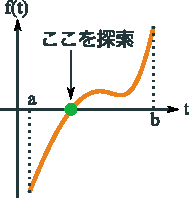
\includegraphics[width=0.8\hsize]{img/brentq.pdf}
        \end{figure}
    \end{minipage}
\end{frame}
\begin{frame}{brentqの注意点}
    \begin{itemize}
        \item a,bの間に解がなければならない
        \item 複数の解があった場合一つしか探索できない
        \item 解はわずかな誤差を含む
    \end{itemize}
\end{frame}

\subsection{全曲率をもとにした取り出し}
\begin{frame}{曲率・全曲率}
  \begin{description}
    \item[曲率] 軌道の曲がり具合を表す
    \begin{align}
      \kappa(t) = \dfrac{1}{r}
    \end{align}
      軌道の回転が強い(rが小さいほど)大きな値
    \item[全曲率] 軌道がどれだけ曲がったかを示す
    \begin{align}
      \mu(t) = \int_a^b \kappa(s)ds
    \end{align}
    ここで$s$は軌道長
  \end{description}
\end{frame}
\begin{frame}{例: 円の場合}
  \begin{figure}
    \centering
    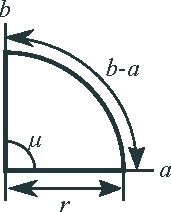
\includegraphics{img/curvature.pdf}
  \end{figure}
\end{frame}

\begin{frame}[standout]
  Questions?
\end{frame}
\end{document}
